\chapter{Weiterentwicklung eines Clients zu einem Messeprototyp}
\label{cha:weiterentwicklung-messeprototyp}
Nach der Entscheidung für die Weiterentwicklung der nativen Android-App, begann die Planung der möglichen Erweiterungen. Dabei wurden besonders Performance- und Stabilitätsaspekte in den Vordergrund gestellt. Darüber hinaus sollte aber auch die Oberfläche einem Messeprototypen entsprechend verbessert werden und Funktionen, die aus den Kann-Kriterien des Pflichtenheftes entspringen, umgesetzt werden, um einen größeren Funktionsumfang präsentieren zu können.

\section{Anpassungen an der Ablauflogik}
\label{sec:anpassungen-ablauflogik}
Die Ablauflogik der nativen App wurde weitestgehend beibehalten, da die Planung im Vorfeld schon eine komplette \textit{User-Story} vorgesehen hat. So muss man sich zuerst anmelden, um dann durch die Trainingspläne und Übungen navigieren zu können und abschließend die Möglichkeit hat ein Training einzutragen. Demnach sind in diesem Sinne keine Verbesserungen oder Änderungen sinnvoll.\\
Aufgrund dessen wurden Anpassungen vorgenommen, die nach Außen nicht sichtbar sind, die Stabilität und die Leistungsfähigkeit der App aber zu einem sehr großen Teil verbessert haben. So wurde die Synchronisation aus den Methoden der \textit{Get}- und \textit{Post}-Abfragen extrahiert und zentralisiert (Vergleich dazu in Kapitel \ref{ssec:cache-unsere-funktionsweise}).\\
Die Funktionalität des \textit{Caches} wurde nur hinsichtlich der Synchronisation mit dem Server angepasst.  Darüber hinaus wurden keine Änderungen vorgenommen und das Eintragen von Daten erfolgt jeweils beim Abrufen von Server-Daten, sowie beim Übertragen von Daten zum Server.
%Sequenzdiagramm-RecentOnline
\begin{figure}[h]
\centering
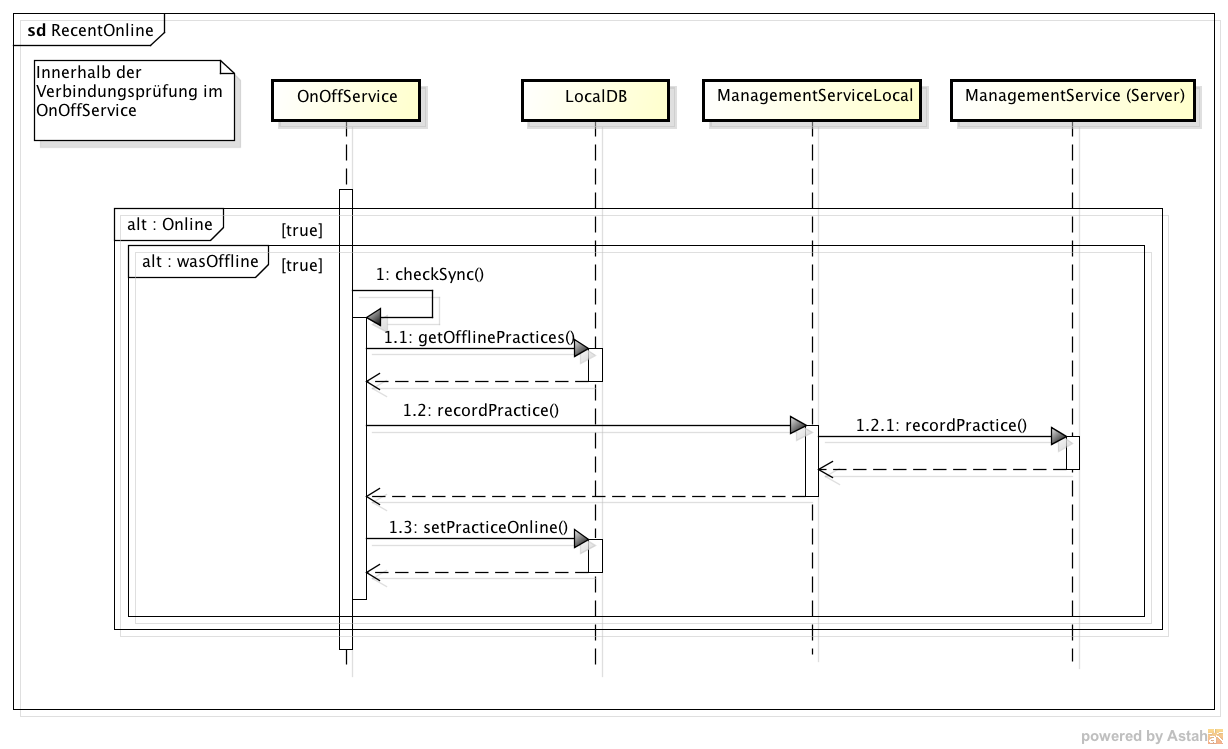
\includegraphics[width=\linewidth]{content/images/fITNat-RecentOnline}
\caption{Squenzdiagramm \textit{RecentOnline}}
\label{pic:nat-RecentOnline}
\end{figure}
Die Abbildung \ref{pic:nat-RecentOnline} verdeutlicht den neuen Ablauf des Synchronisierens. Bedingung zum Start des Synchronisierens ist die Tatsache, dass die Applikation aktuell eine Verbindung zum Server besitzt und im vorhergehenden Status noch \textit{offline} war. Falls dann im Vorfeld Daten angelegt wurden, die nur lokal gespeichert werden konnten, werden diese im Falle des Synchronisierens ausgelesen, auf dem Server gespeichert und in der lokalen Datenbank wieder als "zum Server synchronisiert" gekennzeichnet.\\
In diesem 2. Meilenstein wurde der Programmcode refaktorisiert, um die Umsetzung weiterer Funktionen zu erleichtern. Im Folgenden ist es nunmehr nötig die Daten, die während der Zeit im \textit{Offline}-Modus angelegt wurden, in der Methode \textit{checkSync()} einzutragen.\\
Unter der vorherigen Architektur hätte die Logik in jede Verbidnungs-Operation kopiert werden müssen und hätte somit zu einer großen \textit{Code}-Redundanz geführt. Diese Redundanz sollte unbedingt umgangen werden und deshalb ist diese zentralisierte Stelle zum Überprüfen der zu übetragenden Daten umgesetzt worden.

\section{Anpassungen an der Oberfläche}
\label{sec:anpassungen-oberflaeche}
Die Oberfläche wurde soweit angepasst, dass ein durchgängige \textit{Corporate Design} erkennbar ist. Die Oberfläche, insbesondere \textit{Buttons} und Dialoge wurden in diesem Schritt angepasst.\\
Dabei wurden zwei \textit{Designs}, jeweils für den Login- und den Registrieren-\textit{Button}, umgesetzt. Dazu war es nötig eine \ac{XML}-Datei anzulegen, die dann die Eigenschaften der Schaltfläche zu beschreiben hat (Quellcode \ref{lst:BtnSignInNotClicked}):
\lstinputlisting[caption=Design des Login-\textit{Buttons}, label=lst:BtnSignInNotClicked, style=xml]{content/listings/ButtonSignInStyle.xml}\\
Weiterhin wurden die Dialogfenster mit Animationen versehen, um eine zum Betriebssystem passende \textit{Usability} gewährleisten zu können. Dazu musste ähnlich zum \textit{Button} eine \ac{XML}-Datei angelegt werden und darin dann die Bewegungen des Fensters beschrieben werden (Quellcode \ref{lst:slideRight}).
\lstinputlisting[caption=Dialog-Animation, label=lst:slideRight, style=xml]{content/listings/slide_right.xml}\\
Weiterhin wurden die \textit{Icons} zur Kenntlichmachung des Verbindungsstatus gegen zum Design passende ausgetauscht und ein App-\textit{Icon} eingefügt.

\section{Implementierung der Statistik}
\label{sec:implementierung-statistik}
Um Fortschritte des Nutzers anzeigen zu können, wurde eine Übersicht mit den eingetragenen Trainingsleistungen implementiert. Diese ist für jede Übung über einen längeren Klick auf das Übungs-Feld erreichbar. In dem Balkendiagramm ist das Produkt aus dem Trainingsgewicht, der Wiederholungszahl und der Satzzahl dargestellt.\\
Zur Darstellung wird die \textit{Xamarin-Extension BarChart} verwendet. Das Paket wird in das Projekt eingebunden und kann durch einen einfachen Aufruf mit der Übergabe eines Daten-\textit{Arrays} verwendet werden (Quellcode: \ref{lst:statistik}).\\
Zur Generierung der Diagramm-Daten waren Informationen über die Übung, den Trainingsplan und den \textit{User} nötig. Diese Daten werden über einen \textit{Intent} an die \textit{StatisticActivity} übergeben, in welcher dann die benötigten Daten abgerufen werden.
\lstinputlisting[caption=Statistik \textit{Activity}, label=lst:statistik, style=sharpc]{content/listings/StatisticActivity.cs}

\section{Fazit aus Meilenstein 2}
\label{sec:fazit-meilenstein-2}
Zusammenfassend kann festgehalten werden, dass der zweite Meilenstein zur Optimierung der nativen Adnroid-Applikation beigetragen hat. So konnte durch das Auslagern der Synchronisation Last vom dem \textit{UIThread} genommen werden. Die daraus folgenden Vorteile wurden bereits in Kapitel \ref{cha:native-app} vorgestellt.\\
Das es sich am Ende der Entwicklung um einen Messeprototypen handeln soll, ist das Design von besonderem Interesse. Diese Anforderung wurde im ersten Meilenstein zurückgestellt, um zuallererst einen Fokus auf den technischen Vergleich legen zu können. Nach der Sondierung der besseren Möglichkeit sollte diese dann weiter ausgebaut werden. Deshalb hat diese App eine Verbesserung der Oberflächen erhalten.\\
Die Statistik (ein Kann-Kriterium aus \ref{sec:Pflichtenheft}) wurde zusätzlich umgesetzt, da das Interesse an der Umsetzung eines langen Klicks und der Möglichkeiten der \textit{BarChart-Extension} groß waren.\\
Abschließend kann festgehalten werden, dass der zweite Meilenstein der nativen Applikation die letzten Verfeinerungen zum Prototypen gegeben hat.